\author{Philipp Dominik Bzdok}

\title{Bachelorarbeit Medientechnologie \linebreak \linebreak
Authentifizierungsmethoden für digitale Fernsignaturen auf Grundlage der Handy-Signatur}

\documentclass[11pt,a4paper,ngerman]{scrreprt}
\usepackage[T1]{fontenc}
\usepackage{fontspec}
\usepackage[ngerman]{babel}

\usepackage{fancyhdr}
\pagestyle{fancy}
\fancyhf{}
\setlength{\headheight}{14pt}
\fancyhead[R]{\textsl{\rightmark}}
\fancyfoot[R]{\thepage}

\fancypagestyle{plain}{%
    \renewcommand{\headrulewidth}{0pt}%
    \fancyhf{}%
    \fancyfoot[R]{\thepage}%
}
\addtokomafont{disposition}{\rmfamily}

\usepackage[style=alphabetic,backend=biber]{biblatex}
\addbibresource{Literaturverzeichnis.bib}

\usepackage{color}
\usepackage{tabularx}
\usepackage{booktabs}
\usepackage{amsmath}
\usepackage{amssymb}
\usepackage{graphicx}
\usepackage[skip=5pt,font=footnotesize]{caption}
\usepackage{csquotes}
\usepackage{enumitem}

\usepackage{todonotes}

\usepackage[titles]{tocloft}
\newlistof{listing}{lol}{Quellcodeverzeichnis}

\usepackage[newfloat]{minted}
\usemintedstyle{xcode}
\setminted[java]{linenos,tabsize=2,breaklines,fontsize=\footnotesize,frame=lines,framesep=2ex,autogobble}
\setminted[ruby]{linenos,tabsize=1,breaklines,fontsize=\footnotesize,frame=lines,framesep=2ex,autogobble}

\usepackage[bookmarksnumbered]{hyperref}
\hypersetup{pdfborder={0 0 0}, breaklinks=true}
\usepackage{bookmark}

\setlength{\parskip}{0.5em}
\setlength{\parindent}{0em}

\setlength{\cftlistingnumwidth}{3em}

\newcommand{\ruby}[1]{\mintinline{ruby}{#1}}

% !TEX root = Bachelorarbeit_Philipp_Bzdok

\begin{document}
\maketitle

% ----------------------------------------------------------------
% Preamble DE
% ---------------------------------------------------------------- 
\chapter*{Bachelorarbeit}
\textbf{Thema:}

Authentifizierungsverfahren für digitale Fernsignaturen auf Grundlage der Handy-Signatur
\\[4ex]
\textbf{Gutachter:}
\begin{enumerate}
    \item Prof. Dr.-Ing. Luigi Lo Iacono (Technische Hochschule Köln)
    \item Dipl.-Ing. Tobias Wagner (n-design GmbH)
\end{enumerate}
\textbf{Zusammenfassung:}

Die digitale Signatur stellt ein wichtiges Werkzeug der modernen Informationstechnik dar und durch Fernsignaturen ist es heutzutage möglich, digital, rechtsgültige Unterschriften zu leisten. Der Prozess der Signatur setzt dementsprechend eine starke Authentifizierung des Benutzers voraus. In diesem Kontext wird die SMS-TAN, das erste Authentifizierungsverfahren der österreichischen Handy-Signatur und das am weitesten verbreitete Zwei-Faktor Authentifizierungsverfahren, analysiert. Darauf aufbauend werden alternative Authentifizierungsverfahren für den Anwendungsbereich Fernsignatur evaluiert. Durch die prototypische Implementierung der TOTP und U2F Authentifizierungsverfahren wird gezeigt, wie mit überschaubarem Aufwand die unsichere SMS-TAN substituiert werden kann um somit ein höheres Sicherheitsniveau zu erreichen.
\\[4ex]
\textbf{Stichwörter:}

Authentifizierung, digitale Signatur, Kryptographieverfahren, SMS-TAN, TOTP, U2F
\\[4ex]
\textbf{Datum:}

\today
\clearpage

% ----------------------------------------------------------------
% Preamble EN
% ---------------------------------------------------------------- 
\chapter*{Bachelors Thesis}
\textbf{Title:}

Authentication procedures for digital remote signatures based on mobile phone signatures
\\[4ex]
\textbf{Reviewers:}
\begin{enumerate}
    \item Prof. Dr.-Ing. Luigi Lo Iacono (Technische Hochschule Köln)
    \item Dipl.-Ing. Tobias Wagner (n-design GmbH)
\end{enumerate}
\textbf{Abstract:}

The digital signature is an important tool of modern information technology and with remote signatures it is now possible to provide digital, legally valid signatures. Accordingly, the signature process requires a strong authentication of the user. In this context, the SMS-TAN, the first authentication procedure of the Austrian mobile phone signature and the most widespread two-factor authentication procedure, is analyzed. Based on this, alternative authentication methods for the field of remote signatures will be evaluated. Through the prototypical implementation of the TOTP and U2F authentication methods, it will be shown how the unsecure SMS-TAN can be substituted with a manageable effort in order to achieve a higher level of security.
\\[4ex]
\textbf{Keywords:}

Authentication, digital signature, cryptographic methods, SMS-TAN, TOTP, U2F
\\[4ex]
\textbf{Date:}

\today
\clearpage

% ----------------------------------------------------------------
% Eidesstattliche Erklärung
% ---------------------------------------------------------------- 
\chapter*{Eidesstattliche Erklärung}
Ich erkläre an Eides statt, dass ich die vorgelegte Abschlussarbeit selbständig und ohne fremde Hilfe verfasst, andere als die angegebenen Quellen und Hilfsmittel nicht benutzt und die den benutzten Quellen wörtlich oder inhaltlich entnommenen Stellen als solche kenntlich gemacht habe.

\vspace{1.5cm}

\_\_\_\_\_\_\_\_\_\_\_\_\_\_\_\_\_\_\_\_\_\_ \\
(Ort, Datum)

\vspace{0.5cm}

\_\_\_\_\_\_\_\_\_\_\_\_\_\_\_\_\_\_\_\_\_\_ \\
(Unterschrift)

\clearpage

% ----------------------------------------------------------------
% Vorwort
% ---------------------------------------------------------------- 
\chapter*{Vorwort}
Hier möchte ich auf die Umstände der Abschlussarbeit eingehen und denen danken, die mir dabei geholfen haben.
\clearpage

% ----------------------------------------------------------------
% Inhaltsverzeichnis
% ---------------------------------------------------------------- 
\tableofcontents
\clearpage

% ----------------------------------------------------------------
% Inhalt
% ----------------------------------------------------------------

\chapter{Einleitung}
Digitale Signaturen nehmen in der heutigen Zeit eine wichtige Rolle in der Informationstechnik und somit im Alltag ein. Mit Hilfe von digitalen Signaturen ist es möglich beliebigen Daten zweifelsfrei Integrität und Authentizität nachzuweisen. Die Eigenschaften der Integrität und Authentizität sind besonders wichtig im juristischen Kontext der elektronischen Signatur, in welchem sie das Gegenstück zur handschriftlichen Unterschrift bildet. Der Begriff \emph{elektronische Signatur} wird oft synonym zur \emph{digitalen Signatur} verwendet, jedoch ist die elektronische Signatur ein juristischer Begriff, welcher erstmals in einem überarbeiteten Entwurf der EU-Richtlinie 1999/93/EG von der EU-Kommission verwendet wurde \cite{eSigEU99}. Der Begriff digitale Signatur hingegen stammt aus der Mathematik beziehungsweise aus der Kryptographie und bezeichnet einerseits ein asymmetrisches Kryptographieverfahren, aber anderseits den mathematischen Wert, welcher durch das Kryptographieverfahren erzeugt wird.

Digitale Signaturen werden bereits in einem breiten Spektrum von Anwendungen eingesetzt, wie zum Beispiel für Verschlüsselung von E-Mail oder Zertifikatsbasierten Systemen. Des weiteren werden digitale Signaturen immer häufiger in neuen Anwendungsbereichen eingesetzt. Eine besondere Anwendung auf die ich im Laufe dieser Ausarbeitung explizit eingehen möchte, ist die österreichische \textit{Handy-Signatur}. Die \textit{Handy-Signatur} ermöglicht es den Bürgern Österreichs sich ohne zusätzliche Hardware wie Kartenlesegeräte online per Handy auszuweisen oder Formulare und Dokumente elektronisch zu unterschreiben \cite{handySigOnline}. Die Besonderheit dieser digitalen Signatur ist, dass die \textit{Handy-Signatur} eine qualifizierte elektronische Signatur auslöst und somit juristisch einer handgeschriebenen Unterschrift gleichgesetzt werden kann. Die für die Signatur benutzte Authentifizierungsmethode ist die mobile \textit{SMS-TAN}. Diese Authentifizierungsmethode wurde jedoch bereits von NIST\footnote{National Institute of Standards and Technology} in ihrer Tauglichkeit eingeschränkt, da SMS nie dafür gemacht worden ist Geheimnisse zu übertragen \cite{mobileSec,NIST800-63B}. Trotz der mangelhaften Eignung von SMS als Kanal für OOB-Authentifizierung\footnote{Out-Of-Band Authentifizierung - Authentifizierung über separaten Kanal}, ist das SMS-OTP\footnote{One time password} die am meisten verbreitete Variante der Multi-Faktor Authentifizierung \cite[Abb. 3]{fido17}.

Aus diesem Grund möchte ich in dieser Arbeit die Eigenschaften der Authentifizierungsmethode der \textit{Handy-Signatur} beleuchten und darauf basierend Alternativen evaluieren und prototypisch implementieren. Mein Ziel ist es, die modernen Möglichkeiten von Multi-Faktor Authentifizierung im Kontext der elektronischen Signatur zu vergleichen und zu bewerten, um abschließend eine Aussage über die Tauglichkeit für den Anwendungsbereich \textit{Fernsignatur} machen zu können.

\section*{Abgrenzung}
Die digitale (Fern-)Signatur besteht aus vielen komplexen Verfahren, wie Hashfunktionen, Kryptographieverfahren, Smartcards, uvm.. Diese möchte ich nur der Vollständigkeit halber erläutern. In diesen Bereichen werde ich mich nur auf bereits veröffentlichte Methodiken stützen und von ihnen Gebrauch machen. Insbesondere setze ich bestimmte Rahmenbedingungen für die Implementierungen der Prototypen voraus, wie gesicherte Übertragunskanäle, sichere Schlüsselerzeugung, sichere Schlüsselspeicherung, sichere Zufallsgeneratoren und sichere Signaturerstellungseinheiten, da diese außerhalb der eigentlichen Authentifizierung fungieren.
\clearpage


\chapter{Grundlagen}
Um die Eignung von Authentifizierungsmethoden bestimmen zu können, müssen erst einmal die Rahmenbedingung festgelegt werden. Die digitale Signatur und die \textit{Handy-Signatur} werden im folgenden beleuchtet, da dies der Anwendungsbereich ist, welchen die Authentifizierungsmethoden schützen sollen. Dazu stelle ich verschiedenste Signaturvarianten und deren Komponenten im Detail dar. Nach der Bestimmung dieser Eigenschaften wird die Authentifizierung im Kontext der Signatur erläutert.

\section{Hash-Funktionen}\label{sec:Hash-Funktionen}
\textit{Hash-Funktionen} spielen eine zentrale Rolle in der Welt der Kryptographie und \textit{digitalen Signaturen}. Allgemein bilden diese Funktionen eine Nachricht beliebiger (Bit-)Länge auf einen Hash-Wert festen Länge ab. Der Hash-Wert ist abhängig von der gesamten Nachricht und sollte möglichst schnell berechnet werden können. Dietmar Wätjen beschreibt die Kollisionsfreiheit als eine besondere Eigenschaft von \textit{Hash-Funktionen} \cite[S. 89]{krypt08}: 
\begin{quote}
    ``Es sei $M$ eine Nachricht. Eine Hashfunktion $h$ ist \emph{schwach kollisionsfrei für $M$} [...], wenn es berechnungsmäßig praktisch unmöglich ist, eine Nachricht $M' \neq M$ mit $h(M) = h(M')$ zu finden. [...]
    Eine Hashfunktion ist \emph{stark kollisionsfrei} [...], wenn es berechnungsmäßig praktisch unmöglich ist, Nachrichten $M$ und $M'$ mit $M' \neq M$ und $h(M') = h(M)$ zu finden.''
\end{quote}
Für die Verwendung von \emph{Hash-Funktionen} im Kontext der Signatur muss die Funktion eine sogenannte \emph{Einweg-Hash-Funktion} sein, wie in \cite[S. 99]{krypt08} beschrieben:
\begin{quote}
    ``Eine Hashfunktion ist eine \emph{Ein-Weg-Funktion} [...], wenn es für einen gegebenen Fingerabdruck $z$ berechnungsmäßig praktisch unmöglich ist, eine Nachricht $M$ mit $h(M)=z$ zu finden.''
\end{quote}
Implizit ergibt sich aus der Forderung nach stark kollisionsfreien \textit{Hash-Funktionen} auch die Eigenschaften der Ein-Weg-Funktionen \cite[S. 99]{krypt08}.

Die \textit{Hash-Funktionen} sind so wichtig für die \textit{digitalen Signaturen}, da bei den gängigen Signaturvarianten nur der Hash-Wert der Nachricht signiert wird und nicht die Nachricht selbst. Wichtige Funktionen in diesem Kontext, die in ihrer Sicherheit stetig durch führende Institutionen (NIST\footnote{National Institute of Standards and Technology - Secure Hash Standard \cite{shs180-4}}, SOG-IS\footnote{Senior Officials Group Information Systems Security \cite{sogisACM}}/BSI\footnote{Bundesamt für Sicherheit in der Informationstechnik \cite{bsi-tr-02102-1}}, etc.) geprüft werden, sind:
\begin{table}[h]
    \begin{tabularx}{\textwidth}{ lX }
        \toprule
        Familie & Ausprägungen \\ 
        \midrule
        SHA2 & SHA-256, SHA-512/256, SHA-384 und SHA-512 \\
        SHA3 & SHA3-256, SHA3-384, SHA3-512 \\
        \bottomrule
    \end{tabularx}
    \caption{Empfohlene Hash-Funktionen}
    \label{table:Hashfunktionen}
\end{table}

Eine Signatur soll die Eigenschaften Integrität und Authentizität der zu signierenden Daten sicherstellen. Damit die Authentizität gewährleistet werden kann, muss erst die Integrität der Nachricht sicher gestellt werden. An dieser Stelle greifen die Eigenschaften der \textit{Hash-Funktion}. Dadurch, dass nur der Hash-Wert signiert wird, kann der Empfänger der Signatur durch eine eigene Hash-Wert Berechnung der Nachricht nachvollziehen, dass die Nachricht nicht verändert worden ist\footnote{Durch die Änderung der Nachricht würde auch die Signatur ungültig werden}. Außerdem bietet die Signatur des Hash-Wertes mit fixer Länge Laufzeitvorteile in einigen Signaturverfahren.

\section{Digitale Signaturen}
Als \textit{digitale Signatur} bezeichnet man im allgemeinen ein asymmetrisches Kryptosystem\footnote{Oberbegriff für Public-Key-Verschlüsselungsverfahren}. Bei asymmetrischen Kryptographiesystemen besitzt jeder Teilnehmer ein Schlüsselpaar, bestehend aus einem \emph{öffentlichen Schlüssel} und einem \emph{privaten Schüssel}. Der \emph{private Schlüssel} wird für die Signaturerstellung verwendet, wobei der \emph{öffentliche Schlüssel} von einer beliebigen anderen Person abgerufen werden kann, um die Signatur zu verifizieren (siehe Abb. \ref{fig:Signaturablauf}). Da ausschließlich der Teilnehmer selbst Zugang zu seinem eigenen \emph{privaten Schlüssel} hat, eignet sich ein solches System hervorragend zur Sicherstellung von Authentizität von Daten und somit zur \textit{digitalen Signatur}. Authentizität ist eine der fünf wichtigen Eigenschaften einer Signatur \cite{sch05}:
\begin{enumerate}
    \item Sie ist \textbf{authentisch}. Das bedeutet, dass der Unterzeichner die Signatur willentlich ausgeführt hat.
    \item Sie ist \textbf{fälschungssicher}. Das bedeutet, dass die Signatur ausschließlich vom Unterzeichner ausgeführt worden ist und von niemand anderen.
    \item Sie ist \textbf{nicht wiederverwertbar}. Das bedeutet, dass die Signatur nur auf einer Nachricht gültig ist.
    \item Die signierte Nachricht ist \textbf{unveränderbar}. Das bedeutet, dass die Nachricht nach der Signatur nicht modifiziert werden kann.
    \item Die Signatur ist \textbf{bindend}. Das bedeutet, das der Unterzeichner diese zu einem späteren Zeitpunkt nicht annullieren oder bestreiten kann.
\end{enumerate}
\clearpage
\begin{figure}[h]
    \centering
        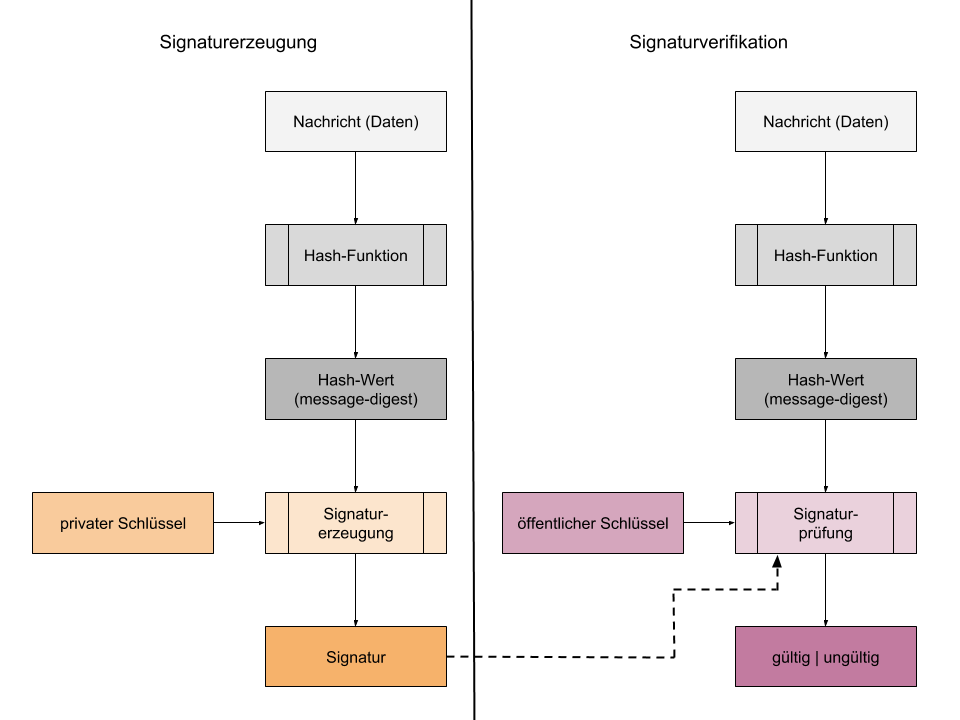
\includegraphics[width=\textwidth]{Abbildungen/Ablauf_Signatur.png}
    \caption{Schematischer Ablauf der Signaturerzeugung und Verifikation}
    \label{fig:Signaturablauf}
\end{figure}

Es gibt Grundsätzlich zwei Arten eine Nachricht $M$ digital zu signieren, wobei $S$ und $V$ zwei Personen sind \cite[S. 28-29]{kryptSec11}:
\begin{enumerate}
    \item Signatur mit Nachrichten-Rückgewinnung: Die Nachricht $M$ wird ohne Vorverarbeitung mit dem \emph{privaten Schlüssel} $d_s$ von $S$ signiert, sodass die daraus resultierende Signatur die Form $s = f_{d_s}(M)$ hat. Diese Nachricht kann von $V$ wiederum durch den \emph{öffentlichen Schlüssel} $e_s$ von $S$ dechiffriert und die ursprüngliche Nachricht wiederhergestellt werden: $M = f_{e_s}(f_{d_s}(M))$. Nur geeignet für Nachrichten kürzer als die Schlüssellänge.
    \item Signatur mit Hash-Wert Anhang: Die Nachricht $M$ wird mit Hilfe einer Hash-Funktion\footnote{Siehe Abschnitt \ref{sec:Hash-Funktionen}} $h(M)$ auf einen Wert mit konstanter Länge (z.B. 160 Bit) abgebildet. Die Signatur hat somit die Form $s = f_{d_s}(h(M))$ und wird zusätzlich zur Nachricht übertragen. Die Person $V$ kann nun den Hash-Wert der Nachricht $M$ durch $h(M) = f_{e_s}(f_{d_s}(h(M))$ errechnen. Auch geeignet für längere Nachrichten.
\end{enumerate}
In der Praxis findet nur die Signatur mit Hash-Wert Anhang Verwendung, da sonst die Signatur linear mit der Größe der Nachricht wächst. Welche Signaturalgorithmen $f_{d_s}(h(M))$ in der Praxis verwendet werden, wird hauptsächlich über den fortlaufend aktualisierten ``Digital Signature Standard (DSS)'' des National Institute of Standards and Technology in den USA vorgegeben. Dieses Dokument stellt Empfehlungen dar, welche Signaturalgorithmen als sicher angesehen werden können und wie diese zu verwenden sind. Auf europäischer Ebene veröffentlicht die SIG-IS Crypto Working Group das sogenannte ``SOG-IS Crypto Evaluation Scheme Agreed Cryptographic Mechanisms'' \cite{sogisACM}.

Auf Grundlage der Empfehlung der SOG-IS möchte ich zur Übersicht die gängigen Signaturverfahren aufzählen:
\subsection{RSA}
Der \textbf{R}iverst-\textbf{S}hamir-\textbf{A}dleman Algorithmus ist ein Public-Key Kryptosystem und findet oft Anwendung in Bereichen der Verschlüsselungsverfahren. Jedoch kann dieser Algorithmus auch zur Signatur von Nachrichten eingesetzt werden. 
\begin{quote}
    ``Die Sicherheit von RSA basiert auf der Schwierigkeit, große Zahlen in ihre Primfaktoren zu zerlegen.'' \cite[S. 82]{ertel12}
\end{quote}
\subsubsection{Schlüsselerzeugung}
Zwei stochastisch unabhängige Primzahlen $p$ und $q$ werden generiert, wobei $p \neq q$. Die beiden Primzahlen sollten so groß gewählt werde, dass das RSA-Modul $n=p \cdot q$ die gewünschte Stellenlänge hat. Das Schlüsselpaar besteht aus $e$ (encrypt) und $d$ (decrypt) und wird mit Hilfe der Eulerschen Funktion ermittelt:
\[
    \Phi(n = p \cdot q) = (p-1) \cdot (q-1)
\]
Einer der beiden Schlüssel wird zufallsmäßig gewählt, sodass er kleiner ist als $\Phi(n)$ und teilerfremd zu $\Phi(n)$ ist. Der andere Schlüssel ergibt sich aus der Bedingung für RSA, dass die beiden Schlüssel $e$ und $d$ eines Paares multiplikativ invers in der Arithmetik modulo $\Phi(n)$ sind:
\[
    e \cdot d \equiv \bmod \Phi(n) 
\]
Der \emph{private Schlüssel} $d$ ist geheim und muss durch spezielle Maßnahmen geschützt werden, da er für die Signatur benutzt wird. Der \emph{öffentliche Schlüssel} $e$ und der Modulo $n$ werden veröffentlicht und dienen zur Verifikation der Signatur. Die Primzahlen $p$ und $q$ müssen ebenfalls sicher verwahrt werden. Sie können aber auch vernichtet werden um Missbrauch vorzubeugen.
\subsubsection{Signaturerzeugung}
Voraussetzung für die Signaturerzeugung, ist die Formatierung\footnote{RSA-Padding} des Hash-Wertes auf die Länge des Moduls $n$. Die Signatur $s$ für die Nachricht $M$ kann nun berechnet werden durch:
\[
    s = (M^d) \bmod n    
\]
\subsubsection{Signaturverifikation}
Die Signatur kann wiederrum unter Kenntnis des \emph{öffentlichen Schlüssels} bestehend aus $(e, n)$ verifiziert werden:
\[
    (s^e) \bmod n = (M^d)^e \bmod n = M'
\]
Falls die wiederhergestellte Nachricht $M'$ mit der übertragenen Nachricht $M$ übereinstimmt, so kann die Signatur als gültig angesehen werden.
\subsubsection{Anmerkungen}
Bei RSA handelt es sich um ein deterministisches Verfahren. In der Praxis wird statt der unmittelbaren Nachricht der Hash-Wert dieser Nachricht signiert. In diesem Fall muss $m$ mit $h(m)$ ersetzt werden. Besonders die Erzeugung der Zufallszahlen und der \emph{private Schlüssel} sind von besonderer Wichtigkeit und müssen durch spezielle Verfahren geschützt werden, auf die ich in Kapitel \ref{sec:Authentifizierung} noch detailliert eingehen werde.

\subsection{Digital Signature Algorithm (DSA)}
Dieses Signaturverfahren wurde erstmals 1991 vom National Institute of Standards and Technology vorgeschlagen und letztendlich auch im Jahr 1994 als Standard im Digital Signature Standard (DSS) offiziell aufgenommen.
\begin{quote}
    ``Die Sicherheit dieses Verfahrens beruht auf der [..] Schwierigkeit des Diskreten Logarithmenproblems $\mathbb{F}^*_p$.'' \cite[S. 45]{bsi-tr-02102-1}
\end{quote}
Im Gegensatz zu RSA eignet sich dieses Verfahren nicht zur kryptographischen Verschlüsselung von Nachrichten, sondern ist speziell für den Anwendungsbereich der \textit{digitalen Signaturen} eingeführt worden. Ein weiterer Unterschied zu RSA ist die Notwendigkeit einer kryptographischen Hash-Funktion zur Signaturerzeugung.
\subsubsection{Schlüsselerzeugung}
Wähle zwei Zahlen, welche durch den Standard definiert sind und die Sicherheit des Verfahrens vorgeben:
\[
    (L, N) \in \{(1024, 160), (2028, 224), (2048, 256), (3072, 256)\}
\]
Anschließend werden die Primzahlen $p$ und $q$ mit folgenden Eigenschaften erzeugt:
\[
    2^{N-1} < q < 2^N \quad\textrm{,}\quad 2^{L-1} < p < 2^L \quad\textrm{und}\quad q|(p-1)
\]
Zusätzlich wird eine Zahl $\alpha \in \mathbb{F}^*_p$ gewählt und $g$ berechnet:
\[
    g := \alpha^{(p-1)/q} \bmod p
\]
Falls $g = 1$ wiederhole die Berechnung von $g$ mit einem anderen $\alpha \in \mathbb{F}^*_p$. Der letzte Schritt der Schlüsselerzeugung besteht aus der Wahl einer Zahl $x \in \{1, \ldots, q - 1 \}$ und $y := g^x \bmod p$. Der \emph{öffentliche Schlüssel} setzt sich zusammen aus $(p, q, g, y)$ und der \emph{private Schlüssel} aus $x$.

Wie auch bei RSA, wird der \emph{private Schlüssel} zur Signaturerzeugung genutzt und muss geschützt werden. Der \emph{öffentliche Schlüssel} dient wiederum auch der Verifikation der Signatur.
\subsubsection{Signaturerzeugung}
Die Erzeugung der Signatur benötigt eine Hash-Funktion. Dabei sollte eine empfohlene Funktion aus der Tabelle \ref{table:Hashfunktionen} verwendet werden. Der aus der Funktion resultierende Hash-Wert sollte der Bit-Länge von $q$ entsprechen. Ebenso sollte die Länge von $p$ mindestens 2000 betragen\footnote{Bis 2022 als sicher eingestuft.\cite{bsi-tr-02102-1}}.

Zur Berechnung wird noch eine Zufallszahl $k \in \{ 1, \ldots, q - 1 \}$ aus einem kryptographisch sicheren Zufallszahlengenerator benötigt. Diese Zahl wird pro Signatur erzeugt und muss, wie der \emph{private Schlüssel}, sicher verwaltet werden. Die Signatur einer Nachricht $M$ welche durch das DSA Verfahren generiert wird, besteht aus dem Zahlenpaar $r$ und $s$:
\[
    r = (g^k \bmod p)
\]
Zur Berechnung von $s$ muss außerdem eine Zahl $z$ bestimmt werden aus den linkesten $N$ Bits des Hash-Wertes $h(M)$:
\[
    s = (z + xr)k^{-1} \bmod q
\]
Die Signatur, bestehend aus $(s, r)$ kann nun zusammen mit der Nachricht $M$ verifiziert werden.
\subsubsection{Signaturverifikation}
Um die Signatur, bestehend aus $(s, r)$, auf der Nachricht $M$ zu prüfen, bedarf es des \emph{öffentlichen Schlüssels} $(p, q, g, y)$ des Unterzeichners. Im ersten Schritt wird überprüft ob: 
\[
    0 < r < q \quad\textrm{und}\quad 0 < s < q
\]
Falls einer dieser beiden Bedingungen nicht erfüllt werden, ist die Signatur als ungültig anzusehen. Damit die Signatur als gültig angesehen werden kann, muss $v$ berechnet werden durch:
\begin{align*}
    v& = (((g)^{u1}(y)^{u2}) \bmod p) \bmod q \quad\textrm{, mit}\\
    w& = (s)^{-1} \bmod q \\
    z& = \textrm{linkeste N Bits von $h(M)$} \\
    u1& = (zw) \bmod q \\
    u2& = (rw) \bmod q
\end{align*}
Falls $v = r$, ist die Signatur gültig.
\subsubsection{Anmerkungen}
Im Gegensatz zur RSA-Signaturvariante handelt es sich hierbei um einen probabilistischen Algorithmus, da die zufällige Wahl des \emph{privaten Schlüssels} mit $x \in \{1, \ldots, q - 1 \}$ essenziell ist. Wichtige schützenswerte Merkmale dieses Verfahrens sind der \emph{öffentliche Schlüssel} $x$ und die Zufallszahl $k$ aus der Signaturerzeugung. Neben der hier dargestellten Variante des DSA Signaturalgorithmus, gibt es außerdem noch die Variante unter der Verwendung von Elliptischen Kurven (ECDSA).

\section{Mobile Signaturen}\label{sec:MobileSignaturen}
Durch den Entwurf der EU-Richtlinie 1999/93/EG wurde die gesetzliche Grundlage für rechtsverbindliche elektronische Signaturen geschaffen. Die Richtlinie sieht eine Gerüst von Anforderungen für die Technologien rund um die elektronische Signaturen vor, basierend auf einer Zertifizierungstelle\footnote{Auch Certificate Authority oder CA genannt.}, welche die \emph{öffentlichen Schlüssel} zertifiziert und so genannten ``sicheren Signaturerstellungseinheiten'' (SSEE), welche wiederum die \emph{privaten Schlüssel} des Benutzers verwaltet. Die EU-Kommission unterscheidet dabei zwischen der elektronischen Signatur und der \emph{qualifizierten} elektronischen Signatur (QES). Eine QES muss folgende Anforderungen erfüllen \cite{eSigEU99}:
\begin{enumerate}
    \item Sie ist eindeutig einem Unterzeichner zugeordnet.
    \item Sie ist in der Lage, den Unterzeichner zu identifizieren.
    \item Sie wird mit Mitteln erstellt, die der Unterzeichner unter seiner alleinigen Kontrolle hat.
    \item Sie ist mit den Daten, auf die sie sich bezieht, so verknüpft, dass jede spätere Änderung der Daten erkennbar ist.
\end{enumerate}
Die klassische Variante einer SSEE ist die Smartcard, welche mit einem Kartenlesegerät angeschlossen an einem Computer bedient wird und die privaten Schlüssel enthält sowie die mathematischen Operationen einer Signatur durchführen kann. Diese Variante verhindert jedoch die Mobilität des Anwenders und erfordert zusätzliche Hardware, was folglich zu einer schwachen Adaption im privaten Sektor geführt hat. Eine Alternative dazu bieten die \textit{mobilen Signaturen}, welche durch mobile Endgeräte, wie z.B. Mobiltelefone, umgesetzt werden. Nach Rossnagel \cite{rossnagel}, können \textit{mobile Signaturen}   in zwei Varianten klassifiziert werden:
\begin{itemize}
    \item \textbf{Serverseitige mobile Signaturen:} Bei der serverseitigen mobilen Signatur wird die Signatur auf einem (zentralen) Server erstellt. Dazu müssen die kryptographischen Schlüssel auf dem Server verwaltet werden. Der Benutzer muss durch besondere Authentifizierungsmethoden den Zugriff auf diese Schlüssel autorisieren.
    \item \textbf{Clientseitige mobile Signaturen:} Bei der clientseitigen mobilen Signatur wird die Signatur durch ein sicheres Signaturerstellungsgerät (z.B. Smartcard) auf dem Mobilgerät des Benutzers erstellt. Die kryptographischen Schlüssel liegen somit dem Benutzer selbst vor und müssen von diesem sicher verwaltet werden.
\end{itemize}
\subsection{eIDAS}
Die Richtlinie 1999/93/EG der EU-Kommission aus dem Jahre 1999 wurde am 17. September 2014 durch die neue EU-Verordnung Nr.\,910/2014 namens \textit{eIDAS}\footnote{\textbf{e}lectronic \textbf{ID}entification, \textbf{A}uthentication and trust \textbf{S}ervices} aufgehoben. Mit der \emph{eIDAS}-Verordnung wurde auch das Signaturgesetz durch das Vertrauensdientegesetz abgelöst, welches am 29. Juli 2017 in Kraft getreten ist. Außerdem führt die Verordnung das \textit{elektronische Siegel} ein, welches technisch vergleichbar mit der elektronischen Signatur ist. Jedoch ist die elektronische Signatur im wesentlichen eine Willenserklärung und bezieht sich auf eine natürliche Person, während das \textit{elektronische Siegel} sich auf eine juristische Person bezieht und somit als Herkunftsnachweiß dienen kann. ``Es kann überall dort eingesetzt werden, wo eine persönliche Unterschrift nicht notwendig, aber der Nachweis der Authentizität gewünscht ist (z. B. bei amtlichen Bescheiden, Urkunden, Kontoauszügen etc.).''\cite{eu910/2014Website} Ein wesentliches Ziel der \textit{eIDAS}-Verordnung ist die Stärkung des Vertrauens in elektronische Transaktionen, auch über Ländergrenzen den EU hinaus. \cite{eu910/2014}.

Die bereits genannten sicheren Signaturerstellungseinheiten werden von der \textit{eIDAS}-Verordnung zusätzlich als \emph{qualifizierte} Signaturerstellungseinheiten (QSEEs) re-definiert und müssen nach den \textit{Common Criteria} zertifiziert werden um gültige \emph{qualifizierten} elektronischen Signaturen erstellen zu können. Die Anforderungen an eine \emph{qualifizierten} elektronischen Signatur habe sich jedoch nicht geändert, wie in Artikel 26 der \textit{eIDAS}-Verordnung beschrieben \cite[Article 26]{eidasWebsite}.

\section{Handy-Signatur}\label{sec:HandySignatur}
Die \textit{Handy-Signatur} ist ein österreichisches (Fern-)Signaturverfahren und gehört der Gruppe der serverseitigen mobilen Signaturen an. Sie erlaubt es dem Benutzer sich eindeutig im Internet per Mobiltelefon zu authentifizieren. Die Signatur ist eine \emph{qualifizierte} elektronische Signatur und ist der handgeschriebenen Unterschrift per Gesetz\footnote{nach eIDAS-Verordnung} gleichgesetzt. Nach Angaben der A-Trust GmbH, welche für die Entwicklung und die technische Infrastruktur der \textit{Handy-Signatur} zuständig sind, sind aktuell ca. eine Million Nutzer registriert und es werden nach Angaben des Betreibers rund 18.000 Signaturen täglich ausgelöst \cite{atrustHSig}.
\begin{quote}
    ``Egal ob Steuererklärung, Gewerbeanmeldung, Kindergeld-Beantragung, FinanzOnline oder ELGA-Abfragen: Mit der Handy-Signatur können bereits mehrere 100 Formulare digital unterschrieben werden. Amtswege und andere Rechtsgeschäfte, die die eindeutige Personenidentifikation erfordern, sind so an 365 Tagen im Jahr, 24 Stunden am Tag, möglich. Die UserInnen sind nicht mehr an die begrenzten Öffnungszeiten von Ämtern, Banken und Unternehmen gebunden.

    Im Zuge der digitalen Transformation wird eine sichere Authentifizierung im Internet immer wichtiger, um eine verlässliche Identifikation von Personen und Organisationen ortsunabhängig und länderübergreifend zu ermöglichen.'' \cite{atrustHSig}
\end{quote}
Da es sich bei der \textit{Handy-Signatur} um eine serverseitige mobile Signatur handelt, hat der Benutzer dabei keinen direkten Zugriff auf das Schlüsselpaar, welches zur Erzeugung der Signatur nötig ist. Dieses wird stattdessen von der A-Trust GmbH verwaltet. Das Auslösen der qualifizierten elektronischen Signatur über das Online-Portal läuft wie folgt ab (siehe Abb.~\ref{fig:HandySignaturablauf} \cite[S.~3]{mobQes}):
\begin{enumerate}
    \item Benutzer greift auf eine Web-basierte Schnittstelle eines Service Providers zu.
    \item Service Provider schickt standardisierte Signaturanfrage an A-Trust.
    \item Über eine Web-Schnittstelle der A-Trust GmbH gibt der Benutzer seine Mobilfunknummer und sein Passwort ein und versendet sie über eine gesicherte HTTPS-Verbindung an A-Trust.
    \item Eine Transaktionsnummer (TAN) wird von A-Trust an den Mobilfunkanbieter des Benutzers gesendet.
    \item Die TAN wird vom Mobilfunkanbieter an den Benutzer weitergeleitet.
    \item Die TAN wird vom Benutzer über eine gesicherte Verbindung zu A-Trust übertragen.
    \item Signaturerstellung wird von A-Trust durchgeführt und eine standardisiertes Ergebnis an den Service Provider gemeldet.
    \item Service Provider meldet das Ergebnis an den Benutzer über die Web-Schnittstelle.
\end{enumerate}
\begin{figure}[htbp]
    \centering
        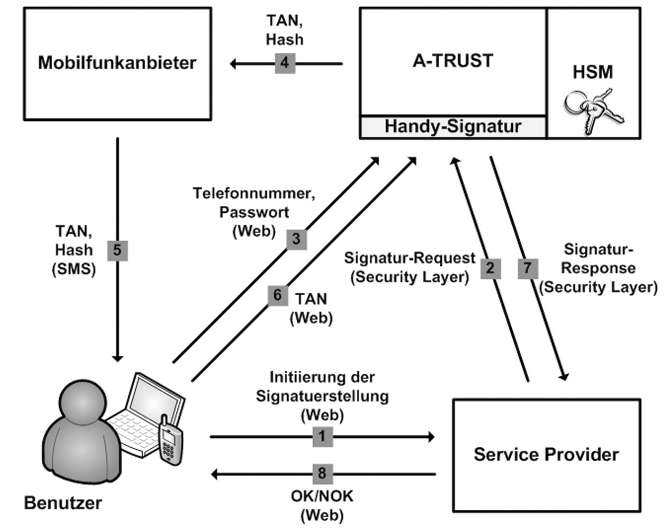
\includegraphics[width=\textwidth]{Abbildungen/Ablauf_Handy-Signatur.png}
    \caption{Schematischer Ablauf der Handy-Signatur}
    \label{fig:HandySignaturablauf}
\end{figure}

Dabei ist zu beachten, dass dieser Vorgang nicht vom gleichen Endgerät ausgeführt werden soll, welches die SMS erhalten hat, da sonst keine \emph{qualifizierte} elektronische Signatur erstellt werden kann. Das Sicherheitskonzept der Anwendung basiert auf der Kombination von üblicher Passwortauthentifizierung und der \emph{Out-Of-Band Authentifizierung} als zweitem Faktor. Der Zugriff auf den \emph{privaten Schlüssel} zur Signaturerstellung muss also erstens durch ein Passwort und zweitens durch den separaten Kanal des Mobilfunknetzes, autorisiert werden. Die eigentliche Signaturerstellung wird von A-Trust in einem zentralem HSM\footnote{Hardware Sicherheits-Modul} vorgenommen, welches die kryptographischen Schlüssel des Benutzers sicher verwahrt.
\subsubsection{Vorteile}
Der Vorteil der Anwendung, gegenüber der Verwendung der Chipkarte (Bürgerkarte), ist die Verwendung des SMS-TAN als Authentifizierungsmethode, statt eines Kartenlesegerätes am Computer des Benutzers. Somit soll eine maximale Verfügbarkeit der Anwendung sichergestellt werden, da die SMS-TAN von beliebigen Mobiltelefonen mit SIM-Karte empfangen werden kann. Außerdem bietet die \emph{Out-Of-Band Authentifizierung} einen zusätzlichen Schutz, falls der Computer des Benutzers kompromittiert sein sollte. Außerdem kann die Signaturerstellung in einer kontrollierten Umgebung stattfinden und somit auch einfacher und effizienter abgesichert werden.
\subsubsection{Nachteile}
Genau in der Tatsache, dass der Authentifizierungscode über eine SMS empfangen wird, liegt auch der größte Nachteil des Verfahrens. Während man eine Chipkarte gewohnheitsmäßig sicher verwahrt und der Zugriff darauf nur über spezielle Hardware mit einem PIN geschehen kann, ist das Mobiltelefon ein Alltagsgegenstand. Des weiteren ist nicht das Endgerät selbst für den Empfang des Authentifizierungscodes zuständig, sondern die Mobiltelefonnummer welche über die SIM-Karte beim Telekomunikationsdienstleister hinterlegt ist. Da die Mobiltelefonnummer kein sicheres Merkmal von Besitz ist, bekommt das Passwort welches zur Anmeldung im Online-Portal genutzt wird eine hohe Bedeutung. Wer Zugriff auf die Mobiltelefonnummer und das Zugangspasswort erlangt, hat die Möglichkeit im Namen dieser Person rechtskräftige Verträge abzuschließen. Mit modernen Smartphones ist es zudem auch möglich, sowohl die Web-Schnittstelle aufzurufen, als auch die SMS mit der TAN zu empfangen. Somit wird das Sicherheitsniveau der separaten Kanäle wieder reduziert. Zusätzlich ist die Trennung der Kanäle ein Nachteil für den Benutzer, da er die Anwendung nicht vom Smartphone benutzen kann sondern diese von einem Computer ausführen muss.

\section{Authentifizierung}\label{sec:Authentifizierung}
Als \emph{Authentifizierung} bezeichnet man den Nachweis einer behaupteten Eigenschaft einer Entität. Diese Entität kann beispielsweise eine Person oder ein Dokument sein. Das verwandte Wort \emph{Authentifikation} bezeichnet hingegen die Prüfung der Echtheit der Eigenschaft.
\begin{quote}
    ``Bei der Authentifikation gibt es zwei Rollen: Die eine Partei, die ihre Identität nachweisen will (Beweisende, ``prover'') und die andere Partei, die den Beweis nachprüft (Verifizierende, ``verifier''). Das Wort \emph{authentisieren} bezeichnet die beweisende Rolle und das Wort \emph{authentifizieren} bezeichnet die verifizierende Rolle. Mit dem Wort \emph{Authentifikation} werden beide Rollen zusammengefasst. Der Sprachgebrauch ist jedoch nicht ganz einheitlich.'' \cite[S. 149]{kryptSec11}
\end{quote}
\subsection{Methoden}
Die Methoden der Authentifizierung können in drei Kategorien eingeteilt werden:
\begin{description}[font=\rmfamily]
    \item[Wissen:] Eine Person kann sich durch das Wissen einer bestimmten Information gegenüber einer zweiten Partei authentisieren. Für die Authentifizierung durch Wissen sind in der Regel keine Hilfsmittel notwendig, da sie auf immateriellem Gut basiert. Jedoch hat dies auch Nachteile, wie z.\,B. dass Informationen vergessen, vervielfältigt oder erraten werden können. Beispiele für Authentifikation anhand von Wissen sind:
    \begin{itemize}
    \item Passwort
    \item PIN
    \item Sicherheitsfrage
    \end{itemize} 
    \item[Besitz:] Durch die Verwendung eines Besitztums kann sich eine Person gegenüber einer zweiten Partei authentisieren. Besitz ist immer etwas materielles und kann deshalb nicht einfach vervielfältigt werden. Der Besitzer muss jedoch die sichere Verwahrung sicherstellen, da der Gegenstand sonst verloren gehen oder sogar gestohlen werden könnte. Es liegt auch in der Verantwortung des Besitzers den Gegenstand, mit dem er sich authentisiert, nicht weiterzugeben. Beispiele von Authentifikation durch Besitz sind:
    \begin{itemize}
        \item Schlüssel
        \item USB Stick
        \item Smartcard
        \item Zertifikat
        \item Transaktionsnummer (TAN)
        \item Einmalpasswort (OTP)
    \end{itemize}
    \item[Körperliches Merkmal / Biometrie:] Durch Merkmale des Benutzers selbst kann dieser sich gegenüber einer zweiten Partei authentisieren. Biometrische Merkmale sind in der Regel öffentliche Informationen, wie Gesichts- oder Augenmerkmale, die der Benutzer immer mit sich trägt. Diese Eigenschaften können nicht weitergegeben werden, benötigen für die Erkennung jedoch in den meisten Fällen spezielle Technik. Außerdem kann die Erkennung nur mit einer Gewissen Wahrscheinlichkeit erfolgen, da sich die Merkmale im Laufe der Zeit verändern können. Beispiele von Authentifikation durch Biometrie sind:
    \begin{itemize}
        \item Fingerabdruck
        \item Gesichtserkennung
        \item Stimmerkennung
        \item Iriserkennung
        \item Handschrift
        \item Erbinformationen
        \item Tippverhalten
    \end{itemize}
\end{description}
Durch eine Kombination von den obigen Authentifizierungsmethoden entsteht eine sogenannte \emph{starke Authentisierung}. Ein gängiges Beispiel für eine Zwei-Faktor Authentifikation ist ein Geldautomat: Durch den Besitz der Chipkarte und das Wissen der PIN kann eine Authentifikation in zwei Stufen durchgeführt werden.

Die Authentifizierung im Kontext digitale Signaturen hat einen besonderen Stellenwert, da durch die Signatur rechtsverbindliche Verträge unterzeichnet werden können. Zum Schutz der kryptographischen Schlüssel, welche zur Signaturerstellung notwendig sind, wird die \emph{starke Authentisierung} implementiert. Dazu muss sich der Benutzer, im Falle der Handy-Signatur, der A-Trust GmbH gegenüber mit Passwort (Wissen, erster Faktor) und SMS-TAN (Besitz, zweiter Faktor) authentisieren. Der Faktor der SMS-TAN hat noch die besondere Eigenschaft des separaten Kanals und bietet somit eine Erweiterung des Sicherheitsniveaus.

\subsection{Vergleich}
Die oben genannten Authentifizierungsmethoden werden im folgenden in den Kategorien \emph{Benutzerfreundlichkeit}, \emph{Komplexität} und \emph{Sicherheit} im Kontext der serverseitigen mobilen Signatur verglichen. Die Kategorie Benutzerfreundlichkeit wurde gewählt, da in erster Linie der Benutzer eine Authentisierung durchführen muss. Die Kategorie Komplexität hingegen dient zur Analyse der technischen Umsetzungsmöglichkeiten. Im Anschluss wird die Sicherheit der Verfahren verglichen, wobei die Ergebnisse der Kategorien Benutzerfreundlichkeit und Komplexität eingehen werden.
\subsubsection{Benutzerfreundlichkeit}
Die Marktanalyse der FIDO Alliance \cite{fido17} zeigt eindeutig, dass die Authentifizierung durch Wissen (insbesondere Passwörter) deutlich verbreiteter ist als die übrigen Methoden. Authentifizierung durch Passwörter und PIN sind heutzutage überall anzutreffen und nicht mehr wegzudenken. Diese Adaption zeigt eindeutig, dass sich diese Authentifizierungsmethode in Bezug Benutzerfreundlichkeit ebenfalls durchsetzen kann. Für diese Methode braucht der Benutzer im idealfall keinerlei Hilfsmittel. Die Biometrische Authentifikation ist ebenfalls, aus Sicht des Benutzers, unkompliziert und erfordert keine Hilfsmittel. Lediglich das Gerät an welchem der Benutzer die Authentifizierung durchführen möchte muss die Technik dafür bereitstellen, z.\,B. der Fingerabdrucksensor des Smartphones. Stehen diese technischen Vorraussetzungen jedoch nicht zur Verfügung, muss der Benutzer eine Alternative wählen oder die entsprechende Hardware zur Verfügung stellen. Das wiederum verringert die Benutzerfreundlichkeit dieser Methode. Grundsätzlich ist die Authentifizierung durch Besitz, die Methode mit der geringsten Benutzerfreundlichkeit, da der Benutzer diesen für die Anwendung anschaffen und verwalten muss. 

Zusammenfassend werden die Eigenschaften der Authentifizierungsmethoden im Bezug zur Benutzerfreundlichkeit in Tabelle \ref{table:Benutzerfreundlichkeit} verglichen.
\begin{table}[htbp]
    \begin{tabularx}{\textwidth}{ lXX }
        \toprule
        Methode & Vorteile & Nachteile \\ 
        \midrule
        Wissen & Benutzer Benötigt keine Hilfsmittel & Kann vom Benutzer vergessen werden \\
         & immateriell & Eventuell schwierig sich viele Passwörter zu merken \\
        \midrule
        Besitz & Kann bekannter Gegenstand sein (z.\,B. Chipkarte) & Muss sicher verwahrt werden, da materiell \\
         & & Anschaffung (Kosten) \\
         & & Kann verloren gehen \\
         & & Kann gestohlen werden \\
        \midrule
        Biometrie & Merkmale trägt Benutzer immer bei sich & Merkmale sind öffentliche Informationen \\
         & & Gerät muss Funktionalität bereitstellen \\
        \bottomrule
    \end{tabularx}
    \caption{Vergleich der Benutzerfreundlichkeit von Authentifizierungsmethoden}
    \label{table:Benutzerfreundlichkeit}
\end{table}
\subsubsection{Komplexität}
Die Komplexität einer Authentifizierungsmethode hängt im Wesentlichen vom Maß der Sicherheit ab, welche diese bietet. Jedoch spielen auch andere Faktoren eine große Rolle, wie z.\,B. die Varianz der Eingangsparameter und die Verfügbarkeit von Hardware und Software. Ein Beispiel für eine Authentifizierungsmethode mit geringer Komplexität ist die Passwortauthentifizierung (Wissen). Dieses Verfahren stützt sich auf die sichere Übertragung und der sicheren Speicherung des Passwortes, da der Benutzer vorgibt wie sicher das Passwort ist. Eine wichtige Komponente der Authentifizierung durch Wissen sind die in Kapitel \ref{sec:Hash-Funktionen} beschriebenen Hash-Funktionen, da das Wissen welches zur Authentisierung nötig ist, gesichert\footnote{gesichert im Sinne von nicht wiederherstellbar} gespeichert werden muss.

Im Gegensatz zur Authentifikation mit Wissen, sind die Authentifikation mit Besitz und Biometrie wesentlich komplexer. Die Authentifikation mit Besitz, setzt bestimmte Hardware vorraus, z.\,B. Chipkarten, USB-Sticks oder Mobiltelefone, welche nach bestimmten Spezifikationen gefertigt sein müssen. Außerdem muss die Kommunikation mit diesen Komponenten mit speziellen Protokollen erfolgen. Ebenfalls ist die Komplexität der biometrischen Authentifikation komplexer, da spezielle Verfahren, Software und Hardware eingesetzt werden müssen um Merkmale des Benutzers zuverlässig erkennen zu können. Die Varianz der Eingangsparameter einer biometrischen Authentifikation ist ebenfalls enorm, so können z.\,B. die Eigenschaften des Gesichts oder die Beleuchtungssituation sich verändern. Insgesamt ist die Passwortauthentifizierung die am wenigsten komplexe Variante, gefolgt von der Authentifikation durch Besitz und abschließend ist die Authentifikation durch Biometrie die komplexeste Methode, wie in Tabelle \ref{table:Komplexität} dargestellt.
\begin{table}[htbp]
    \begin{tabularx}{\textwidth}{ lXX }
        \toprule
        Methode & Vorteile (geringe Komplexität) & Nachteile (hohe Komplexität) \\ 
        \midrule
        Wissen & Nur (Text-)Zeichen auf Benutzer-Ebene & Sichere Speicherung \\
         & & Sichere Übertragung \\
        \midrule
        Besitz & Kann bekannter Gegenstand sein (z.\,B. Chipkarte, Mobiltelefon) & Muss bestimmte Sicherheitsanforderungen erfüllen \\
         & & Zugriff über spezielle Protokolle \\
         & & Fertigung \\
        \midrule
        Biometrie & & Varianz der Prüfungsparameter \\
         & & Spezielle Client-Software \\
         & & Spezielle Client-Hardware \\
        \bottomrule
    \end{tabularx}
    \caption{Vergleich der Komplexität von Authentifizierungsmethoden}
    \label{table:Komplexität}
\end{table}
\subsubsection{Sicherheit}
Die wohl wichtigste Eigenschaft der vorgestellten Authentifizierungsmethoden ist die Sicherheit. Diese ist je nach Methode unterschiedlich stark und beeinflussbar. Allgemein kann man sagen, dass keine Authentifizierungsmethode hundert-prozentig sicher ist, jedoch ergeben sich je nach Anwendungsfall unterschiedliche Anforderungen an das Sicherheitsniveau der Authentifizierungsmethode. Im Kontext der mobilen serverseitigen Signatur steht die Sicherheit des kryptographischen Schlüssels im Mittelpunkt. Da durch diesen rechtsverbindliche Verträge geschlossen werden können, muss dieser bestmöglich gesichert werden. In Tabelle \ref{table:Sicherheit} möchte ich eine Sammlung von gängigen Authentifizierungsmethoden \cite{fido17} darstellen und eine Übersicht im Kontext der Sicherheit bieten:
\begin{description}[font=\rmfamily]
    \item[Wissen:] Die meist genutzte Authentifizierungsmethode, die Authentifizierung mit Wissen ist ebenfalls die schwächste, da sie anfällig gegen Abschrift ist. Diese Eigenschaft ermöglicht diverse Möglichkeiten der Kompromittierung, da das Wissen grundsätzlich anfällig gegen Weitergabe und Diebstahl ist. So ein Angriff kann z.\,B. der Diebstahl eines Laptops, auf dem der Benutzer die Passwörter vieler Systeme gespeichert hat, ein Brute-Force Angriff auf ein Passwort, Phishing\footnote{Angriff indem der Benutzer auf einer gefälschten Internetseite sein Passwort eingibt} oder sogar das entziffern eines verschlüsselten Passwortes in einer Datenbank sein. Ein weiterer sehr wichtiger Faktor ist der Benutzer selbst, da dieser effektiv die Sicherheit der Passwörter vorgibt. Da eine Person heutzutage oft auf vielen Plattformen angemeldet ist, muss sie sich dem entsprechend viele Passwörter merken. Jedoch benutzen viele Personen ähnliche oder gleiche Passwörter für verschiedene Internetseiten oder Services, sodass ein potenzieller Angreifer sobald er ein Passwort herausgefunden hat, diesen auf eine Reihe von anderen Internetseiten verwenden kann. Ein Passwort kann also nur so stark sein wie der Benutzer es entwirft, dass bedeutet das er für jede Internetseite oder Service ein einmaliges und starkes\footnote{z.\,B. durch ein Passwortgenerator} Passwort wählen muss, da sonst die Sicherheit dieser Authentifizierungsmethode sehr gering ist.
    \item[Besitz:] Authentifizierung mit Besitz ist besonders komplex in Hinsicht auf die Sicherheit, da der Besitz eines Gerätes oft nur eine Schlussfolgerung ist und nicht direkt geprüft werden kann. Der Geräte-Fingerabdruck durch Cookies und andere Marker ist kein sicheres Merkmal von Besitz eines Gerätes, da prinzipiell ein solches Gerät ohne das Wissen des Besitzer durch Fernsteuerung oder Diebstahl gesteuert werden kann. Eine Alternative implementieren die Verfahren welche auf Einmal-Passwörtern (OTP's) basieren, wie z.\,B. die Software ``Google Authenticator'' für Smartphones oder die SMS-TAN. Diese Verfahren bieten somit eine erhöhte Sicherheit aber induzieren erhöhte Komplexität und somit auch neue Angriffsvektoren. Hardware-basierte Lösungen oder die Geräte auf denen eine Software-basierte Lösung ausgeführt wird können gestohlen werden. Außerdem eröffnet sich insbesondere bei den Software-basierten OTP's eine Reihe von Schwachstellen, da diese in der Regel auf Geräten ausgeführt werden welche kompromittiert sein könnten. Auch die SMS-TAN ist in dieser Hinsicht anfällig, da eine SMS abgefangen oder weitergeleitet werden kann.
    \item[Biometrie:] Biometrische Authentifizierungsmethoden bieten Vorteile gegenüber den anderen Methoden, indem sie sich auf den Benutzer direkt beziehen und diesen somit Identifizieren können. Jedoch ist die Authentifizierung mit körperlichen Merkmalen eine besondere technische Herausforderung und bringt somit Risiken mit sich. Insbesondere die Erkennung der Merkmale ist an komplexe Hardware und Software geknüpft und somit ist die Sicherheit dieser Verfahren durch Implementierungen dieser eingeschränkt. Außerdem ist es möglich bestimmte Merkmale, wie das Gesicht oder die Stimmte einer Person, aufzunehmen und durch einen Angreifer wiederzugeben.
\end{description}
Vergleicht man die Eigenschaften und Schwachstellen der drei individuellen Methoden, so zeigt sicht, dass alle Schwächen haben. Diese liegen jedoch in sehr unterschiedlichen Eigenschaften der Methoden und müssen im Kontext des Anwendungsbereich eingeschätzt werden. Durch die Bedeutsamkeit einer digitalen Signatur muss eine \emph{starke Authentifikation} implementiert werden, indem mehrere Faktoren sich gegenseitig verstärken und somit ein viel höheres Sicherheitsniveau erreicht werden kann. Eine solche Kombination von Authentifizierungsmethoden nennt sich \emph{Multi-Faktor Authentifizierung}.
\begin{table}[htbp]
    \begin{tabularx}{\textwidth}{ >{\hsize=.7\hsize}X>{\hsize=.3\hsize}XXX }
        \toprule
        Methode & Faktor & Beschreibung & Schwachstellen \\
        \midrule
        Passwort, PIN & Wissen & Fixer Wert, welcher beliebig Kombination von Alphanummerische Zeichen enthält & Kann abgefangen, gestohlen, erraten oder erzwungen\footnote{Brute-Force Angriff} werden \\
        Sicherheitsfrage & Wissen & Frage, welche nur der Benutzer beantworten kann & Kann abgefangen, gestohlen oder erraten werden \\
        \midrule
        Hardware-basiertes OTP & Besitz & Separates Gerät, welches Passwort zur einmaligen Benutzung generiert & Kann abgefangen oder gestohlen werden \\
        Software-basiertes OTP & Besitz & Anwendung auf Endgerät des Benutzers, welches Password zur einmaligen Benutzung erzeugt & Kann abgefangen oder gestohlen (Gerät) werden \\
        SMS-basiertes OTP & Besitz & Passwort zur einmaligen Verwendung empfangen per SMS & Kann abgefangen, mitgelesen (Malware) oder gestohlen (Gerät) werden \\
        Smartcard & Besitz & Eine Karte welche eine SSEE enthält und die PKI nutzt & Kann gestohlen werden \\
        Sicherheitsschlüssel & Besitz & Kompaktes Gerät welches eine SSEE enthält und die PKI nutzt & Kann gestohlen werden \\
        Geräte Fingerabdruck & Besitz & Prozess zur Wiedererkennung von Geräten durch Cookies und anderen Markern & Geräteeigenschaften können emuliert oder Cookies gestohlen werden \\
        \midrule
        Fingerabdruck Scan & Biometrie & Fingerabdruck wird elektronisch oder optisch mit einem registrierten verglichen & Abbild kann gestohlen werden \\
        Iris Scan & Biometrie & Eigenschaften der Augen werden mit registrierten optisch verglichen & Abbild kann gestohlen werden \\
        Gesichtserkennung & Biometrie & Eigenschaften des Gesichts werden mit einem registrierten optisch verglichen & Abbild kann gestohlen werden \\
        Stimmerkennung & Biometrie & Eigenschaften der Stimme werden mit einer registrierten akustisch verglichen & Stimme kann aufgenommen (gestohlen) oder simuliert werden \\
    \end{tabularx}
    \caption{Übersicht über gängige Authentifizierungsmethoden}
    \label{table:Sicherheit}
\end{table}


\chapter{Problematik der SMS-TAN}
In diesem Kapitel möchte ich die Authentifizierungsmethode der Handy-Signatur, die \textit{SMS-TAN} näher analysieren und die Schwachstellen dieser Methode im Kontext der serverseitigen mobilen Signatur aufzeigen. Wie bereits in Kapitel \ref{sec:Authentifizierung} dargestellt, handelt es sich bei der \textit{SMS-TAN} um die am weitesten verbreitete Zwei-Faktor Authentifizierung\footnote{In Kombination mit der üblichen Passwortauthentifizierung}. 

\section{SMS-TAN}
Die \textit{SMS-TAN} ist eine Authentifizierungsmethode, welche zur Kategorie der Authentifizierung durch Besitztum gehört. Um diese Methode verwenden zu können muss der Benutzer seine Mobiltelefonnummer im Vorfeld beim Service-Provider registrieren und anschließend bestätigen, wie in Abbildung \ref{fig:SMS-TAN_Registrierung} dargestellt. Jedoch setzt die österreichische Handy-Signatur einen komplexeren Registrierungsprozess um als es in Abbildung \ref{fig:SMS-TAN_Registrierung} dargestellt ist, da der Benutzer eine amtliche Registrierungsstelle aufsuchen oder von seiner bereits registrierten Bürgerkarte gebraucht machen muss. Somit wird die Mobiltelefonnummer, welche die \textit{SMS-TAN} empfängt, direkt an einen registrierten Bürger geknüpft. Das stellt die Grundlage der \emph{qualifizierten} elektronischen Signatur her. Die Transaktionsnummer (TAN) wird für genau eine Anwendung generiert und an den Benutzer, via SMS an sein Mobiltelefon, gesendet. Anschließend kann der Benutzer die TAN auslesen und sie innerhalb einiger Minuten beim Service-Provider\footnote{Google, Amazon, A-Trust, etc. - Meist über eine Web-Schnittstelle} eingeben um sich zu authentifizieren. Die \textit{SMS-TAN} wird in den aller meisten Fällen als Zwei-Faktor Authentifikation zusammen mit einem Passwort verwendet \cite{fido17}. Der typische Use-Case dieser Methode sieht vor, dass der Benutzer sich erst mit einem Passwort authentifiziert bevor er eine SMS mit dem TAN zugesendet bekommt. Somit fungiert die \textit{SMS-TAN} als Einmal-Passwort und wird über den separaten Kanal des Mobilfunknetzes vom Benutzer empfangen. Abbildung \ref{fig:SMS-TAN} zeigt schematisch den Ablauf einer generischen Zwei-Faktor Authentifizierung mit Passwort und \textit{SMS-TAN}. Die Abläufe der Registrierung und der Authentifizierung unterscheiden sich nur im ersten Schritt und bieten dem Benutzer somit eine einfache Methode sich zusätzlich gegen unautorisierte Zugriffe abzusichern. Besonders die \textit{SMS-TAN} als Authentifizierungsmethode erfuhr eine branchenübergreifende Adaption, nicht zuletzt da Mobiltelefone und Smartphones sehr weit verbreitet sind. Nach angaben der Bitkom besitzen im Jahr 2017 78 Prozent aller Deutschen ein Smartphone \cite{bitkomMob} und die Tendenz ist steigend.

Die \textit{SMS-TAN} soll durch das Empfangen mit dem Mobiltelefon das Besitztum des Benutzer verifizieren und somit ein erhöhtes Sicherheitsniveau gegenüber der einfachen Passwortauthentifizierung bieten. In der Theorie trifft dies auch zu, jedoch stellt der Übertragunskanal, die verschiedenen Möglichkeit eine SMS zu empfangen und das Endgerät des Benutzers die Sicherheitseigenschaften der Methode in Frage.
\begin{figure}[htbp]
    \centering
        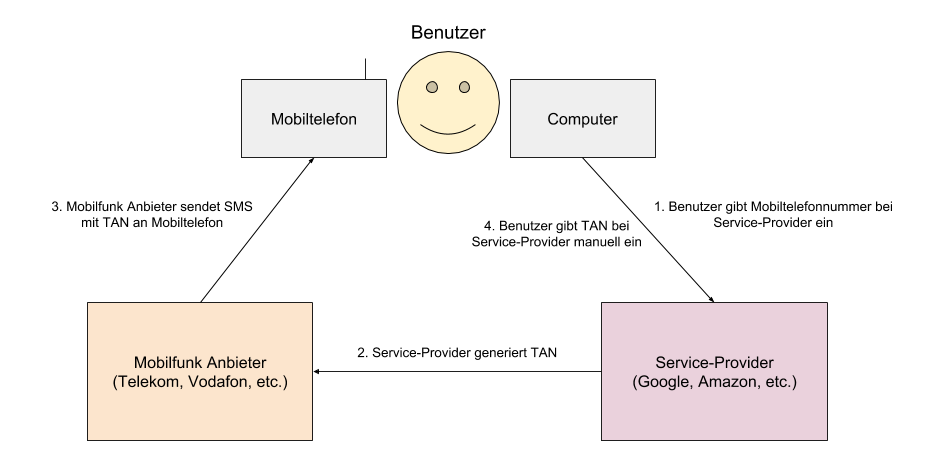
\includegraphics[width=\textwidth]{Abbildungen/Ablauf_SMS-TAN_Registrierung.png}
    \caption{Schematischer Ablauf der SMS-TAN Registrierung}
    \label{fig:SMS-TAN_Registrierung}

    \centering
        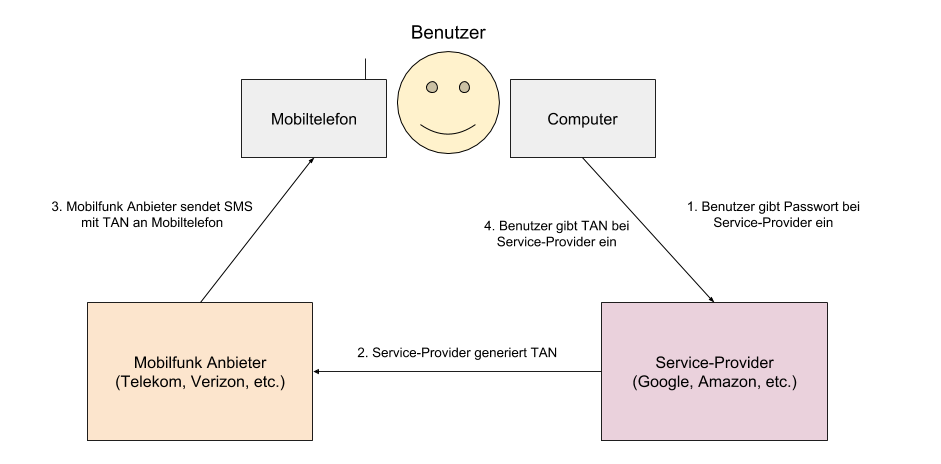
\includegraphics[width=\textwidth]{Abbildungen/Ablauf_SMS-TAN.png}
    \caption{Schematischer Ablauf der SMS-TAN Authentifizierung}
    \label{fig:SMS-TAN}
\end{figure}

\section{Mobiltelefonnummer als Merkmal von Besitz}
Mit der Evolution von ``einfachen'' Mobiltelefonen zu Smartphones ist auch das Risiko für Anwendungen wie der \textit{SMS-TAN} gestiegen. Der Grund dafür ist die zunehmende Vernetzung verschiedenster Geräte wie Smartphones, Tablets, Laptops und Computern. Es ist heutzutage möglich seine SMS nicht nur über sein eigentliches Mobiltelefon zu empfangen, sondern diese an beliege weitere Geräte und Dienste weiterzuleiten. Somit ist der Faktor Besitztum nicht mehr zweifelsfrei durch die Mobiltelefonnummer gegeben und das Sicherheitsniveau der Authentifizierungsmethode sinkt erheblich.

Ein Angriffsvektor auf den Benutzer ist die Mobiltelefonnummer selbst. Ein Angreifer muss keinen physischen Zugriff auf das Mobiltelefon haben um einen Angriff durchzuführen, da die Nachricht welche die TAN enthält an die Telefonnummer gerichtet ist und nicht an das Gerät selbst. Somit könnte ein Angreifer z.\,B. durch \emph{Social Engineering} den Mobilfunkbetreiber überzeugen die Mobiltelefonnummer auf einer neuen SIM Karte zu aktivieren. Diese Vorgehen wir auch \emph{SIM Hijacking} oder \emph{Port-Out Scam} genannt. Selbst T-Mobile warnt auf ihrer offiziellen Seite vor diesem Vorgehen \cite{telekomPortOut}. Der Angreifer gibt sich in diesem Szenario als der Benutzer beim Support des Netzbetreibers aus und behauptet die SIM Karte verloren zu haben, sodass die Telefonnummer auf eine neue SIM Karte überschrieben wird\footnote{Beispielhafte Erfahrung hier zu lesen: https://www.ftc.gov/news-events/blogs/techftc/2016/06/your-mobile-phone-account-could-be-hijacked-identity-thief}. Diese Art von Angriff unterstreicht die Problematik der \textit{SMS-TAN} als Authentifizierungsmethode durch Besitz. Es liegt in der Verantwortung des Netzbetreibers die Telefonnummer des Benutzers zu verwalten und somit ist diese kein Merkmal von Besitz des Benutzers über das Mobiltelefon. Für Angreifer wird es zunehmend einfacher die Mobilfunkbetreiber von einer gefälschten Identität zu überzeugen, da eine Vielzahl von personenbezogenen und vertraulichen Daten bereits durch Hacking-Angriffe auf große Unternehmen wie Equifax\footnote{https://www.ftc.gov/equifax-data-breach} zugänglich gemacht worden sind. Ebenfalls sind Angreifer aus den Reihen der Mobilfunkbetreiber möglich, da diese direkten Zugriff auf die Rufnummerverwaltung ihrer Kunden haben.

\chapter{Alternative Multi-Faktor Authentifizierung}


\chapter{Zusammenfassung}

% ----------------------------------------------------------------
% Quellcodeverzeichnis
% ----------------------------------------------------------------
\clearpage
\phantomsection
\addcontentsline{toc}{chapter}{Quellcodeverzeichnis}
\listoflistings
\clearpage

% ----------------------------------------------------------------
% Tabellenverzeichnis
% ----------------------------------------------------------------
\phantomsection
\addcontentsline{toc}{chapter}{Tabellenverzeichnis}
\listoftables
\clearpage

% ----------------------------------------------------------------
% Abbildungsverzeichnis
% ----------------------------------------------------------------
\phantomsection
\addcontentsline{toc}{chapter}{Abbildungsverzeichnis}
\listoffigures
\clearpage

% ----------------------------------------------------------------
% Literaturverzeichnis
% ----------------------------------------------------------------
\phantomsection
\addcontentsline{toc}{chapter}{Literaturverzeichnis}
\bibliographystyle{ieeetr}
\bibliography{Literaturverzeichnis}

\end{document}